% !TEX program = xelatex
\documentclass[10pt, aspectratio=169]{beamer}

% ── 中文支持 ──
\usepackage{ctex}

% ── 主题与配色 ──
\usetheme{Madrid}
\usecolortheme{whale}
\setbeamertemplate{navigation symbols}{}
\setbeamertemplate{footline}[frame number]
\setbeamerfont{frametitle}{size=\normalsize}

% ── 常用宏包 ──
\usepackage{graphicx}
\usepackage{booktabs}
\usepackage{amsmath,amssymb}
\usepackage{tabularx}
\usepackage{array}
\usepackage{multirow}
\usepackage{pifont}
\usepackage{caption}
\captionsetup[figure]{font=tiny,labelfont=tiny}
\captionsetup[table]{font=tiny,labelfont=tiny}

% ── 全局缩小正文字号，保持内容紧凑 ──
\setbeamerfont{normal text}{size=\small}
\AtBeginDocument{\usebeamerfont{normal text}}

% ── 标题信息 ──
\title{北向资金对A股市场的影响与\\基于北向资金的量化交易策略}
\author{杨明宸}
\institute{清华大学}
\date{\today}

% ══════════════════════════════════════════
\begin{document}

% ── Slide 1: 封面 ──
\begin{frame}
\titlepage
\end{frame}

% ── Slide 2: 研究背景与目标 ──
\begin{frame}{研究背景与目标}
\small
\textbf{研究背景}
\begin{itemize}\setlength\itemsep{1pt}
    \item 沪港通（2014）与深港通（2016）开通以来，北向资金持股总市值超2.3万亿元，日均成交占比10\%--15\%
    \item 市场普遍默认北向资金为"聪明钱"(Smart Money)，但实证证据有限且结论相互矛盾
    \item 现有文献三大缺陷：\textbf{盈利能力度量信息损失}、\textbf{因果识别工具缺位}、\textbf{策略研究存在数据泄露与因子混淆}
\end{itemize}

\vspace{0.3em}
\textbf{核心问题}
\begin{enumerate}\setlength\itemsep{1pt}
    \item 北向资金是否是"聪明钱"？其收益来源于选股还是择时？交易特征如何？
    \item 北向资金对A股\textbf{收益率}和\textbf{波动率}分别产生了什么因果效应？
    \item 能否基于北向资金信息构建独立于动量反转的\textbf{可交易alpha}？
\end{enumerate}

\vspace{0.3em}
\textbf{研究框架}：\; 数据：沪市A股，2017.10--2025.10，逐股日度持仓+行情 \\[2pt]
\centering
\fbox{北向资金特征刻画} $\;\longrightarrow\;$ \fbox{对A股市场影响的因果识别} $\;\longrightarrow\;$ \fbox{量化策略构建与回测}
\end{frame}

% ── Slide 3: 北向资金特征——收益能力与来源分解 ──
\begin{frame}{北向资金特征：收益能力与来源分解}
\small
\begin{columns}[T]
\begin{column}{0.52\textwidth}
\textbf{收益能力验证}
\begin{itemize}\setlength\itemsep{1pt}
    \item 静态持仓绝对收益$\approx 0$，但\textbf{主动交易相对收益}显著为正
    \item 修正相关系数 $\widetilde{Corr}_t$（保留择时信息，不做截面去均值）
    \item HAC稳健t检验：$\hat{\alpha}=0.0021$，$t=3.82$，$p<0.001$ {\color{red}\textbf{***}}
    \item 结论：北向资金通过主动调仓获取显著超额收益
\end{itemize}

\vspace{0.5em}
\textbf{收益来源分解}
\begin{itemize}\setlength\itemsep{1pt}
    \item 选股收益（CsPnl）$\approx$ \textbf{42\%}
    \item 择时收益（TsPnl）$\approx$ \textbf{58\%}
    \item 北向资金的超额收益\textbf{以择时为主导}
\end{itemize}
\end{column}
\begin{column}{0.46\textwidth}
    \centering
    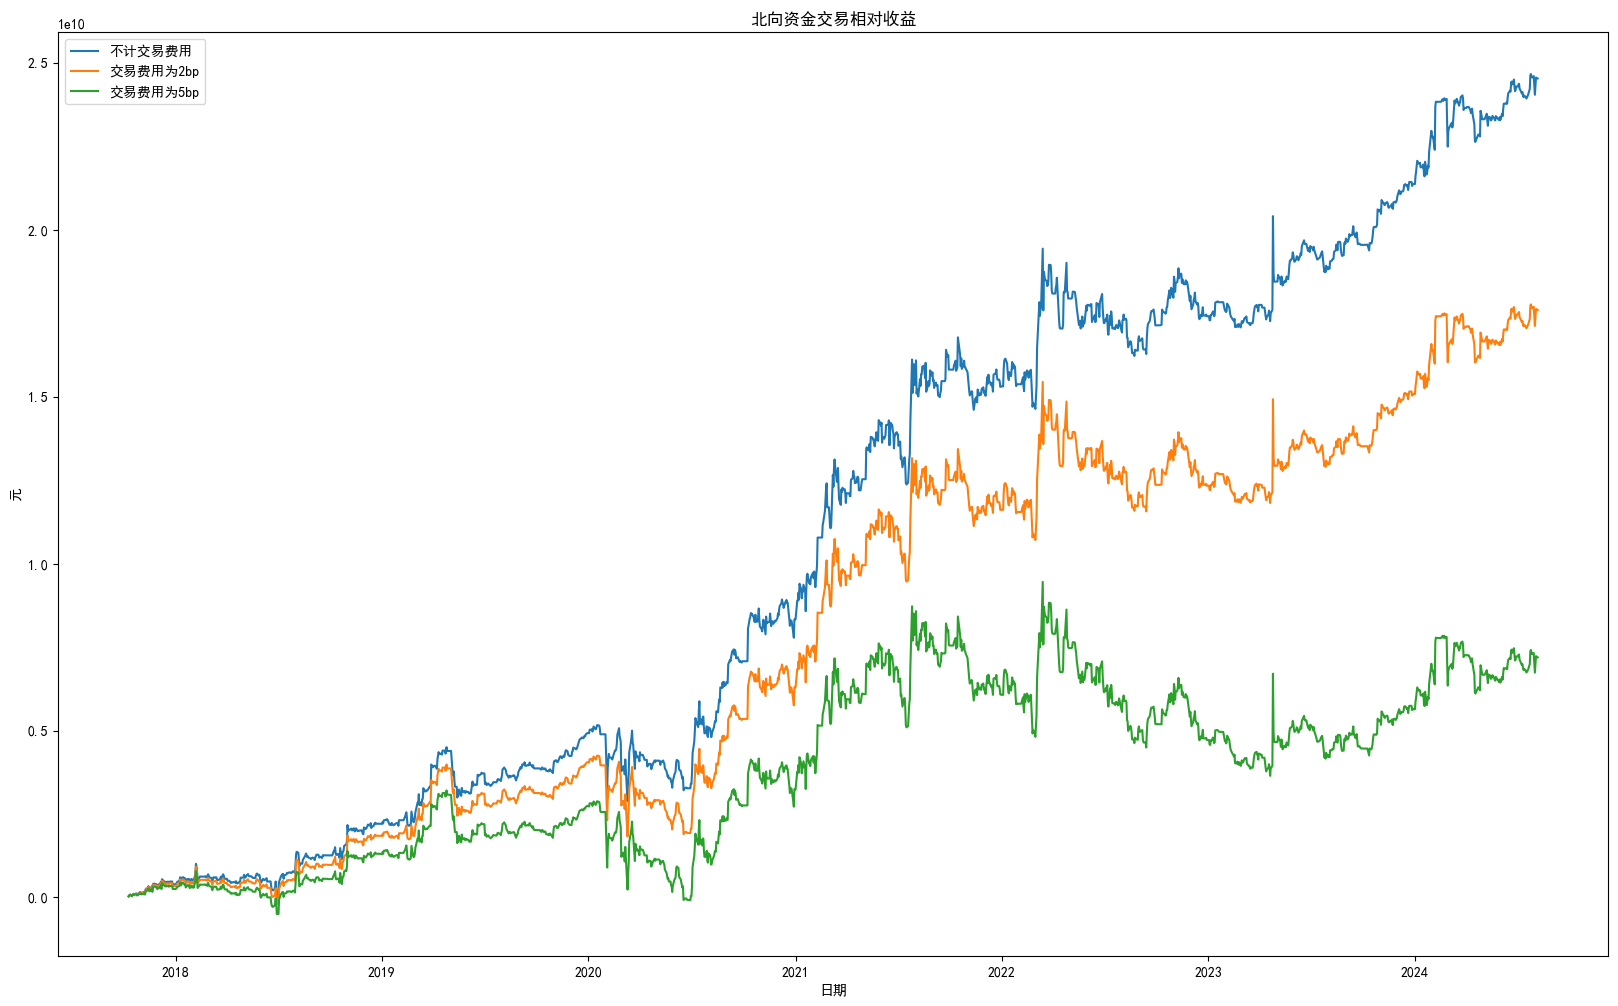
\includegraphics[width=\linewidth,height=0.35\textheight,keepaspectratio]{../Figure/北向交易相对收益.png}
    \vspace{-0.5em}
    {\tiny 北向资金主动交易累积相对收益（多费率情景）}

    \vspace{0.3em}
    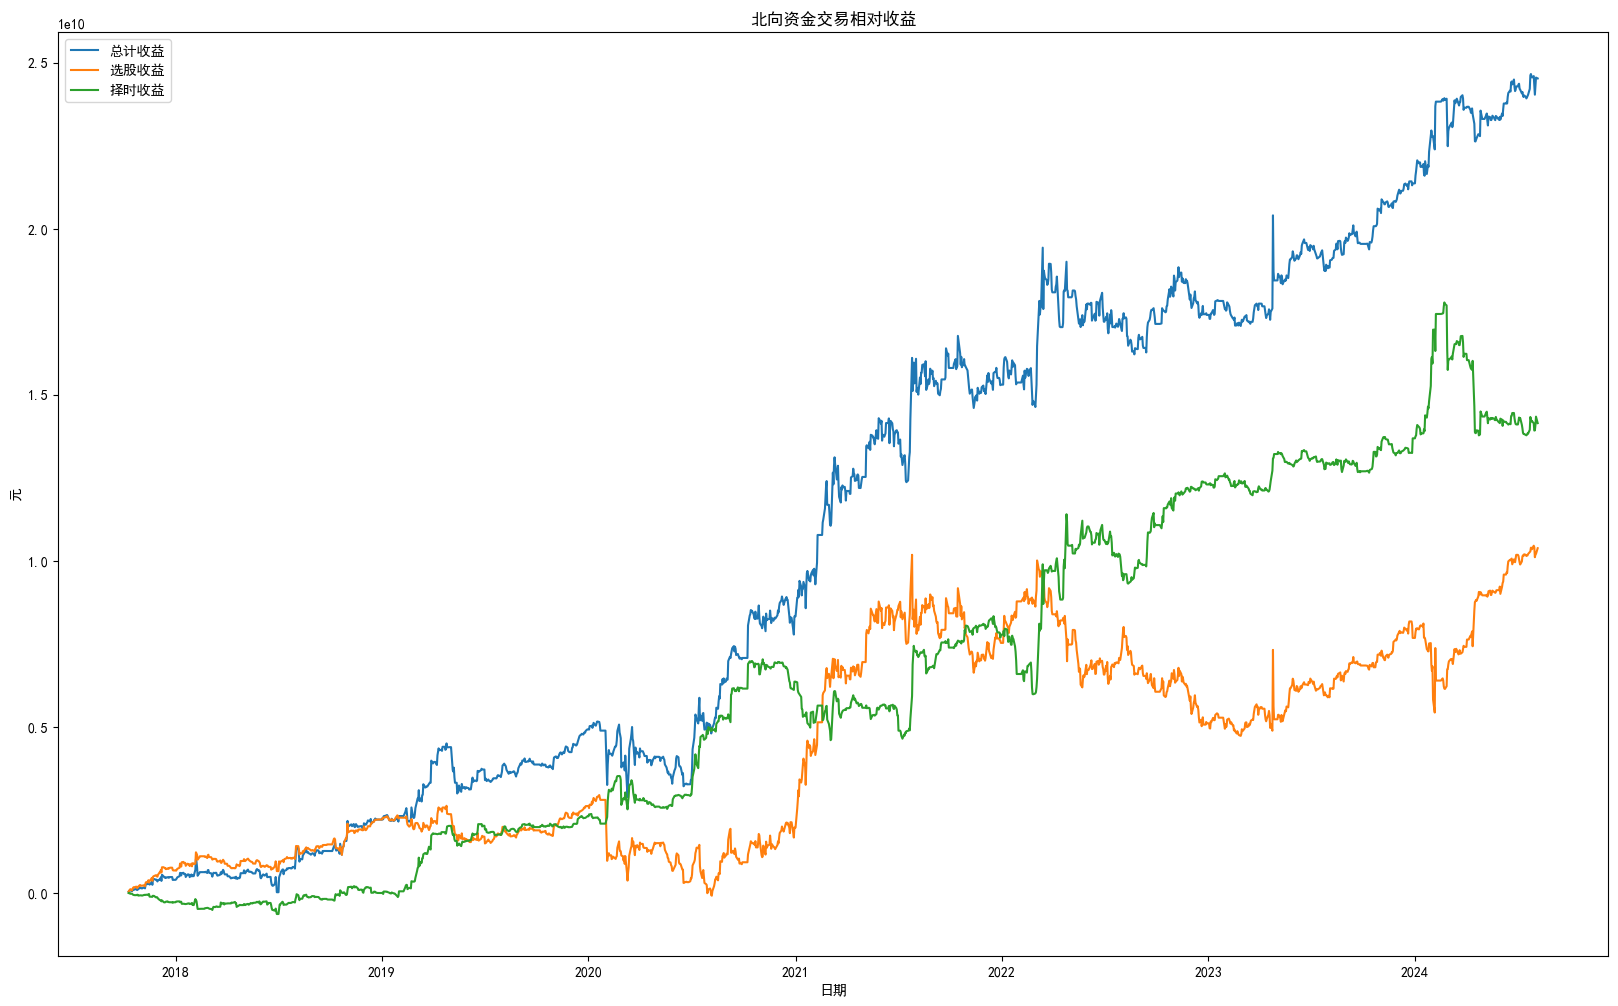
\includegraphics[width=\linewidth,height=0.35\textheight,keepaspectratio]{../Figure/收益分解.png}
    \vspace{-0.5em}
    {\tiny 收益来源分解：选股 vs 择时}
\end{column}
\end{columns}
\end{frame}

% ── Slide 4: 北向资金特征——交易模式与预测期限 ──
\begin{frame}{北向资金特征：交易模式与预测期限}
\footnotesize
\begin{columns}[T]
\begin{column}{0.48\textwidth}
\textbf{交易模式}
\begin{itemize}\setlength\itemsep{0pt}
    \item 构造非对称买卖交易率指标，修正大股东低流动性偏误
    \item 换手率\textbf{远超}机构（1.5$\times$调整后仍显著高出）
    \item 与\textbf{散户}上界相当（4$\times$调整）
    \item $\Rightarrow$\textbf{"对冲基金式"高频交易}特征
\end{itemize}

    \centering
    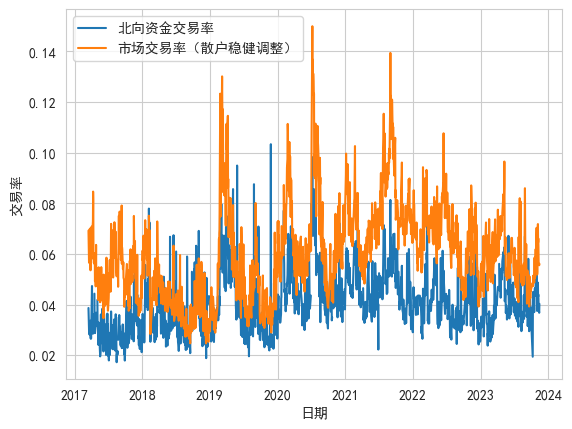
\includegraphics[width=0.88\linewidth,height=0.36\textheight,keepaspectratio]{../Figure/turnover_3.png}
    \vspace{-0.5em}
    {\tiny 北向资金交易率 vs 散户换手率上界（4倍调整）}
\end{column}
\begin{column}{0.50\textwidth}
\textbf{预测能力随期限递减}

\vspace{0.2em}
\centering
{\scriptsize
\begin{tabular}{lccc}
\toprule
\textbf{预测期限} & \textbf{$\bar{\rho}^{(n)}$} & \textbf{NW $t$} & \textbf{显著性} \\
\midrule
1日  & 0.0021 & 3.82 & *** \\
1月 ($n$=21) & 0.0115 & 2.16 & ** \\
1季 ($n$=63) & 0.0188 & 2.69 & ** \\
半年 ($n$=126) & 0.0037 & 0.53 & --- \\
1年 ($n$=252) & $-$0.0010 & $-$0.24 & --- \\
\bottomrule
\end{tabular}
}

\vspace{0.3em}
\raggedright
\textbf{核心发现}：
\begin{itemize}\setlength\itemsep{0pt}
    \item 日频预测能力最强（$t=3.82$）
    \item 月—季度：统计显著但经济意义有限
    \item \textbf{半年及以上：预测力完全消失}
    \item $\Rightarrow$ 信息优势集中于\textbf{短期价格波动}
\end{itemize}
\end{column}
\end{columns}
\end{frame}

% ── Slide 5: 对A股收益率的影响——羊群效应 ──
\begin{frame}{对A股收益率的影响：羊群效应}
\footnotesize
\begin{columns}[T]
\begin{column}{0.48\textwidth}
\textbf{VAR(4)模型 + Granger因果检验}
\begin{itemize}\setlength\itemsep{0pt}
    \item 内生变量：北向净流入 \& 标的股成交额（去趋势）
    \item 北向$\to$成交额：$F=15.44$，$p<0.001$ {\color{red}\textbf{***}}
    \item 成交额$\to$北向：$F=0.64$，$p=0.637$（不显著）
    \item \textbf{单向Granger因果}：北向资金引领市场
\end{itemize}

\vspace{0.3em}
\textbf{脉冲响应函数}
\begin{itemize}\setlength\itemsep{0pt}
    \item 北向净流入冲击后，成交额在\textbf{约4--5个交易日}内显著正向响应
    \item 之后逐步衰减，持续约\textbf{一周}的羊群效应
\end{itemize}

\vspace{0.2em}
\textbf{结论}：北向资金净流入触发内地投资者跟风，引发短期市场联动
\end{column}
\begin{column}{0.50\textwidth}
    \centering
    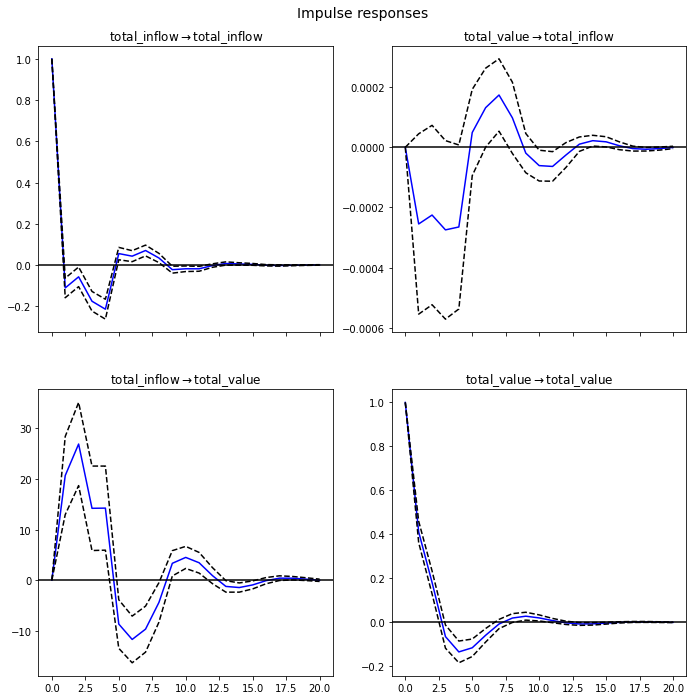
\includegraphics[width=\linewidth,height=0.65\textheight,keepaspectratio]{irf_value.png}
    \vspace{-0.5em}
    {\tiny 北向净流入与标的股成交额的双向脉冲响应函数（VAR(4), 20阶）}
\end{column}
\end{columns}
\end{frame}

% ── Slide 6: 对A股波动率的影响——DID实验设计 ──
\begin{frame}{对A股波动率的影响：双重差分（DID）实验设计}
\small
\textbf{核心问题}：允许北向资金交易是否\textbf{系统性地}改变了标的股票的波动率水平？

\vspace{0.3em}
\begin{columns}[T]
\begin{column}{0.55\textwidth}
\textbf{准自然实验}
\begin{itemize}\setlength\itemsep{1pt}
    \item 事件：2014年11月17日沪港通正式开通
    \item 实验组：首批沪港通标的股（467只，未经纳入/剔出调整）
    \item 对照组：同期未被纳入的沪市A股（280只）
    \item 窗口期：2014.05.17 -- 2015.05.17（前后各6个月）
\end{itemize}

\vspace{0.3em}
\textbf{DID模型}
\begin{equation*}
    \text{Vol}_{i,t} = \alpha_i + \gamma_t + \beta_3\, D_i \times \text{post}_t + \mathbf{X}_{i,t}^{\top}\boldsymbol{\delta} + \varepsilon_{i,t}
\end{equation*}
\begin{itemize}\setlength\itemsep{1pt}
    \item $\alpha_i$：个体固定效应\quad $\gamma_t$：时间固定效应
    \item $\beta_3$（Post$\times$Experiment）：\textbf{核心DID估计量}
    \item 波动率指标：$\text{Vol}_1 = r_{i,t}^2$（日度回报率平方）和 $\text{Vol}_2 = \frac{P^{high}-P^{low}}{P^{open}}$（日内振幅）
\end{itemize}
\end{column}
\begin{column}{0.43\textwidth}
\textbf{识别威胁与应对}
\begin{itemize}\setlength\itemsep{1pt}
    \item \textbf{选择偏误}：标的股系统性偏向大市值蓝筹 $\Rightarrow$ 个体FE吸收
    \item \textbf{时间扰动}：2014--15牛市共同冲击 $\Rightarrow$ 时间FE吸收
    \item \textbf{控制变量}：逐步加入总资产、资产负债率、流动比率、ROA、资产周转率、行业哑变量
\end{itemize}

\vspace{0.3em}
\textbf{稳健性检验}
\begin{itemize}\setlength\itemsep{1pt}
    \item 剔除事件前后各1个月（排除初始建仓暂时性冲击）
    \item 样本量：165,058 $\to$ 136,604
\end{itemize}
\end{column}
\end{columns}
\end{frame}

% ── Slide 7: DID回归结果 ──
\begin{frame}{DID回归结果：核心发现}
\small
\centering

\vspace{-0.3em}
{\scriptsize
\begin{tabular}{lcccccc}
\toprule
& (1) & (2) & (3) & (4) & (5) & (6) \\
\midrule
& \multicolumn{3}{c}{\textbf{Panel A：$\text{Vol}_1$（回报率平方）}} & \multicolumn{3}{c}{\textbf{Panel B：$\text{Vol}_2$（日内振幅）}} \\
\cmidrule(lr){2-4} \cmidrule(lr){5-7}
& 基准 & +财务 & +全部 & 基准 & +财务 & +全部 \\
\midrule
\textbf{Post $\times$ Experiment} & \textbf{0.0040***} & \textbf{0.0039***} & \textbf{0.0039***} & \textbf{9.82e-5***} & \textbf{9.75e-5***} & \textbf{9.76e-5***} \\
& \scriptsize(0.000) & \scriptsize(0.000) & \scriptsize(0.000) & \scriptsize(1.6e-5) & \scriptsize(1.6e-5) & \scriptsize(1.6e-5) \\[0.2em]
Post & 0.0211*** & 0.0210*** & 0.0211*** & 0.0008*** & 0.0008*** & 0.0008*** \\
Experiment & 0.0046*** & $-$0.0038*** & $-$0.0039*** & 9.83e-5 & $-$9.57e-5** & $-$9.19e-5** \\
\midrule
行业哑变量 & 否 & 是 & 是 & 否 & 是 & 是 \\
个体/时间FE & 是 & 是 & 是 & 是 & 是 & 是 \\
财务控制变量 & 否 & 部分 & 全部 & 否 & 部分 & 全部 \\
\midrule
$N$ & 165,058 & 165,058 & 165,058 & 165,058 & 165,058 & 165,058 \\
$R^2$ & 0.320 & 0.320 & 0.320 & 0.136 & 0.136 & 0.136 \\
\bottomrule
\end{tabular}
}

\vspace{0.3em}
\raggedright
\textbf{核心发现}：
\begin{itemize}\setlength\itemsep{1pt}
    \item $\hat{\beta}_3$（Post$\times$Experiment）在\textbf{全部6组设定}中均为正且在\textbf{1\%}水平下高度显著
    \item 系数值对控制变量的加入\textbf{高度不敏感}（0.0039--0.0040），排除遗漏变量偏误
    \item 结论：沪港通标的股在政策开通后波动率\textbf{系统性上升}
\end{itemize}
{\tiny 注：***、**、*分别表示1\%、5\%、10\%显著。括号内为聚类稳健标准误。747只股票，2014.05--2015.05。}
\end{frame}

% ── Slide 8: DID稳健性检验 ──
\begin{frame}{DID稳健性检验：剔除事件临近期}
\small
\centering

\vspace{-0.3em}
{\scriptsize
\begin{tabular}{lcccccc}
\toprule
& (1) & (2) & (3) & (4) & (5) & (6) \\
\midrule
& \multicolumn{3}{c}{\textbf{Panel A：$\text{Vol}_1$}} & \multicolumn{3}{c}{\textbf{Panel B：$\text{Vol}_2$}} \\
\cmidrule(lr){2-4} \cmidrule(lr){5-7}
& 基准 & +财务 & +全部 & 基准 & +财务 & +全部 \\
\midrule
\textbf{Post $\times$ Experiment} & \textbf{0.0034***} & \textbf{0.0033***} & \textbf{0.0033***} & \textbf{6.84e-5***} & \textbf{6.53e-5***} & \textbf{6.55e-5***} \\
& \scriptsize(0.000) & \scriptsize(0.000) & \scriptsize(0.000) & \scriptsize(1.75e-5) & \scriptsize(1.75e-5) & \scriptsize(1.75e-5) \\[0.2em]
Post & 0.0228*** & 0.0226*** & 0.0227*** & 0.0009*** & 0.0009*** & 0.0009*** \\
Experiment & 0.0054*** & $-$0.0049*** & $-$0.0050*** & 0.0001 & $-$0.0001*** & $-$0.0001*** \\
\midrule
行业哑变量 & 否 & 是 & 是 & 否 & 是 & 是 \\
个体/时间FE & 是 & 是 & 是 & 是 & 是 & 是 \\
\midrule
$N$ & 136,604 & 136,604 & 136,604 & 136,604 & 136,604 & 136,604 \\
$R^2$ & 0.320 & 0.320 & 0.320 & 0.141 & 0.141 & 0.141 \\
\bottomrule
\end{tabular}
}

\vspace{0.4em}
\raggedright
\textbf{与完整窗口对比}：
\begin{itemize}\setlength\itemsep{1pt}
    \item 剔除事件前后各1个月后，$\hat{\beta}_3$ 仍在\textbf{1\%}水平下高度显著
    \item $\text{Vol}_1$：点估计下降约15\%--17\%（0.0040$\to$0.0034）
    \item $\text{Vol}_2$：点估计下降约30\%--33\%（9.82e-5$\to$6.84e-5）
    \item \textbf{结论}：波动率上升具有\textbf{持续性}——大部分效应无法归因于初始建仓的暂时性冲击
\end{itemize}
{\tiny 注：样本剔除2014.10.17--2014.12.17全部观测值，仅保留距事件$\geq$1个月的数据。}
\end{frame}

% ── Slide 9: 量化策略设计与回测结果 ──
\begin{frame}{量化策略设计与回测结果}
\footnotesize
\begin{columns}[T]
\begin{column}{0.48\textwidth}
\textbf{策略设计要点}
\begin{itemize}\setlength\itemsep{0pt}
    \item \textbf{目标残差化}："类Barra"框架，剔除市场、行业、市值、动量反转因子 $\Rightarrow$ alpha与动量策略\textbf{统计正交}
    \item \textbf{特征工程}：26个北向资金持仓特征（EMA平滑、排名归一化、回报率残差化）
    \item \textbf{模型}：增量滚动Ridge回归（$\lambda$=0.01，半衰期500日）
    \item 全部预测均为\textbf{真正的样本外}
\end{itemize}

\vspace{0.2em}
\textbf{核心回测指标}

\vspace{0.1em}
\centering
{\scriptsize
\begin{tabular}{ll}
\toprule
年化超额收益 & \textbf{14.518\%} \\
年化夏普比率 & \textbf{4.998} \\
累积平均IC & $\approx$\textbf{0.012} \\
ACF半衰期 & $\approx$\textbf{0.88交易日} \\
\bottomrule
\end{tabular}
}
\end{column}
\begin{column}{0.50\textwidth}
    \centering
    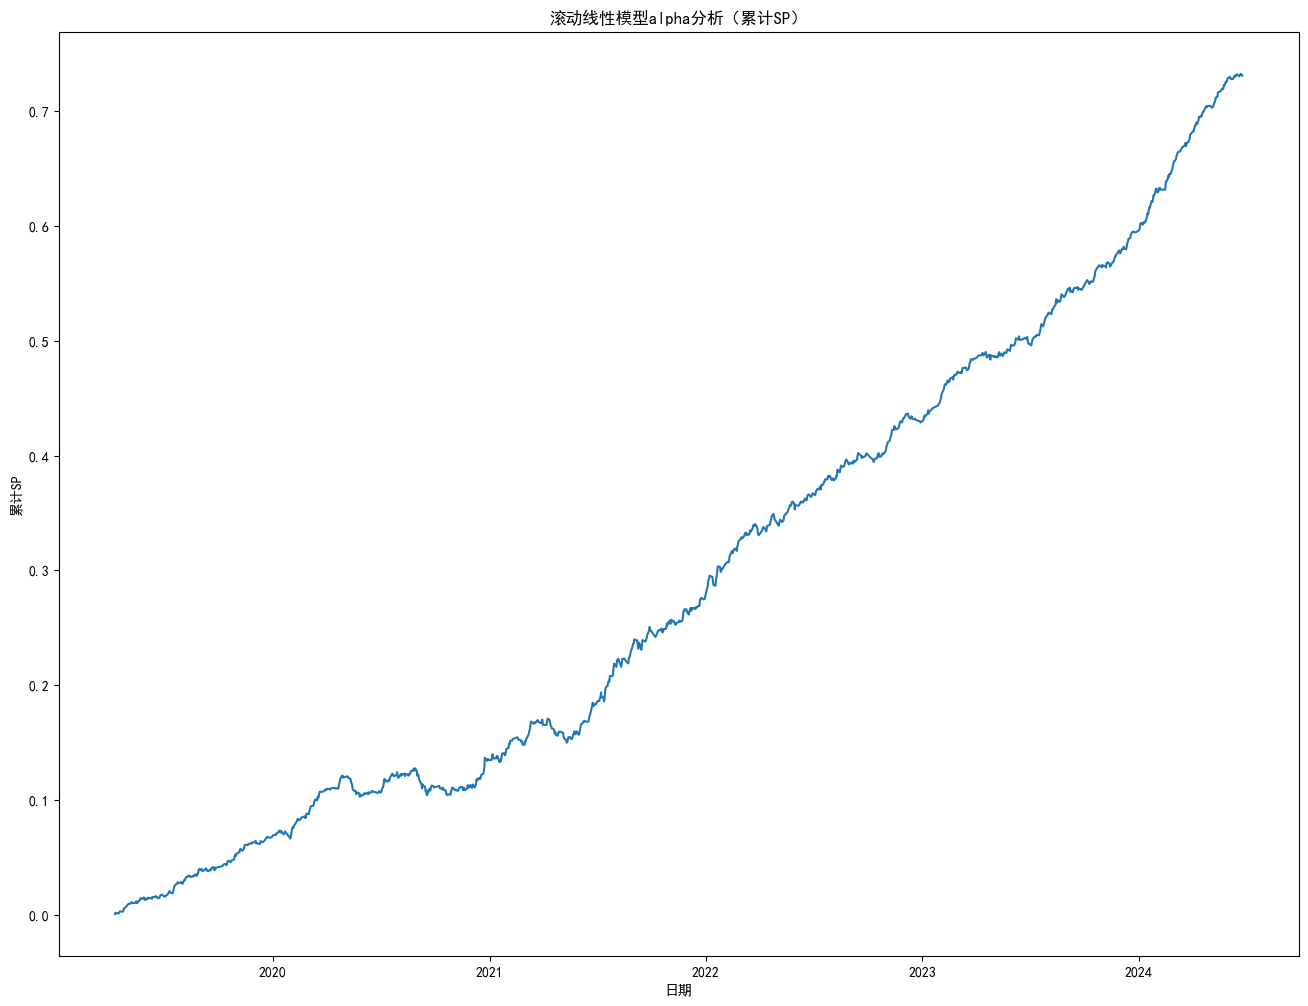
\includegraphics[width=\linewidth,height=0.34\textheight,keepaspectratio]{../Figure/rollingWLS_SP.png}
    \vspace{-0.5em}
    {\tiny 累积平均SP——年化14.5\%，SR$\approx$5.0}

    \vspace{0.2em}
    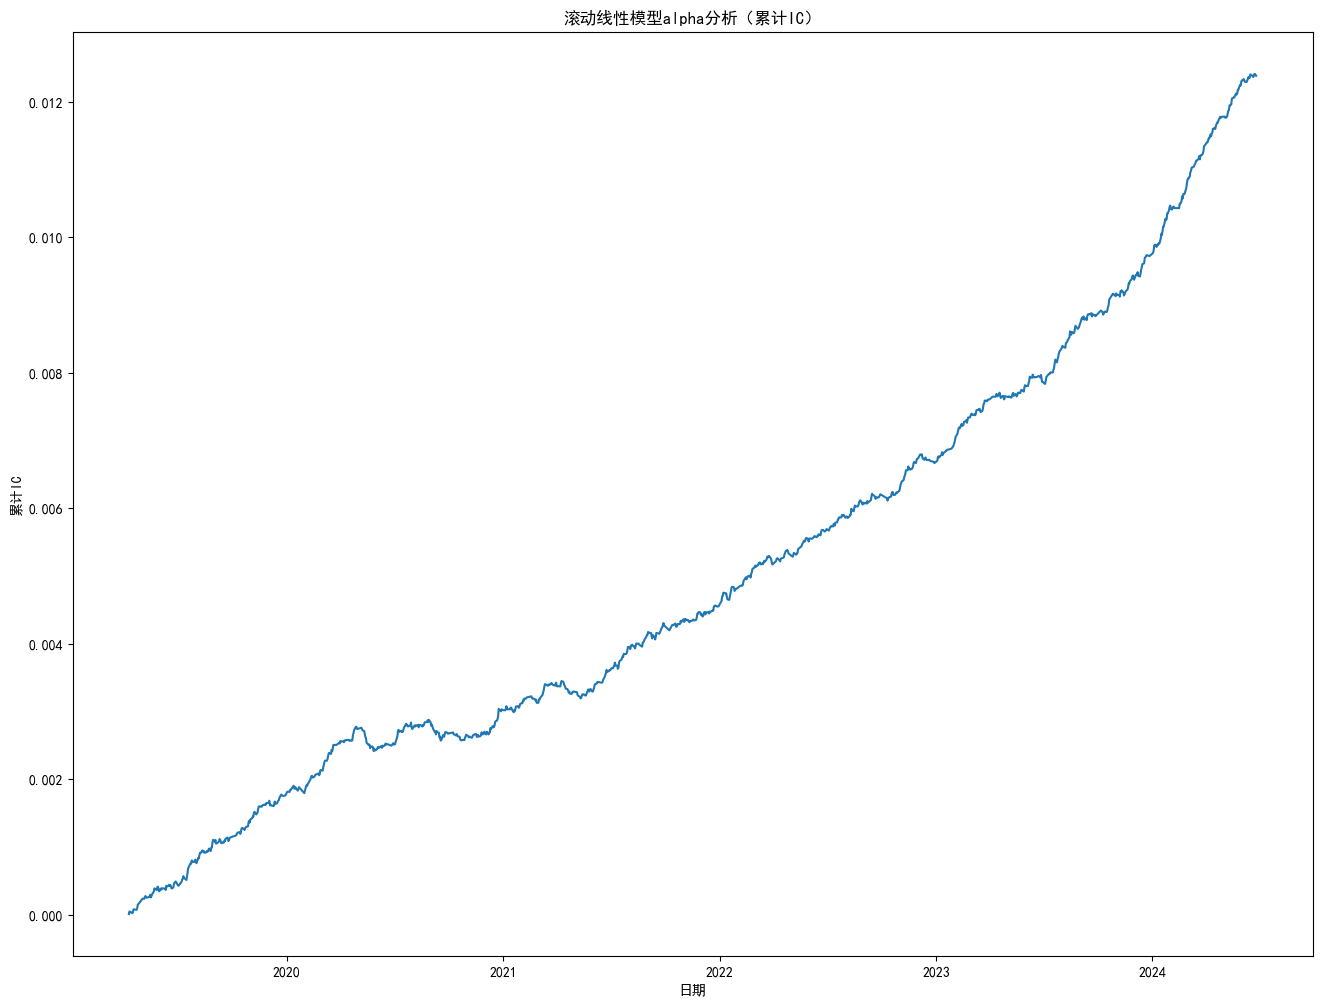
\includegraphics[width=\linewidth,height=0.34\textheight,keepaspectratio]{../Figure/rollingWLS_IC.png}
    \vspace{-0.5em}
    {\tiny 累积平均IC——稳定收敛至$\approx$0.012}
\end{column}
\end{columns}
\end{frame}

% ── Slide 10: 非线性模型对比与总结 ──
\begin{frame}{非线性模型对比与研究总结}
\footnotesize
\begin{columns}[T]
\begin{column}{0.48\textwidth}
\textbf{非线性模型（LightGBM, CatBoost）}
\begin{itemize}\setlength\itemsep{0pt}
    \item 样本内IC \textbf{显著优于}线性基准
    \item 样本外IC增益\textbf{几乎为零}
    \item 原因：低信噪比+共线性+有效样本不足
    \item \textbf{结论}：alpha可预测成分\textbf{主要为线性结构}
\end{itemize}

    \centering
    \vspace{0.1em}
    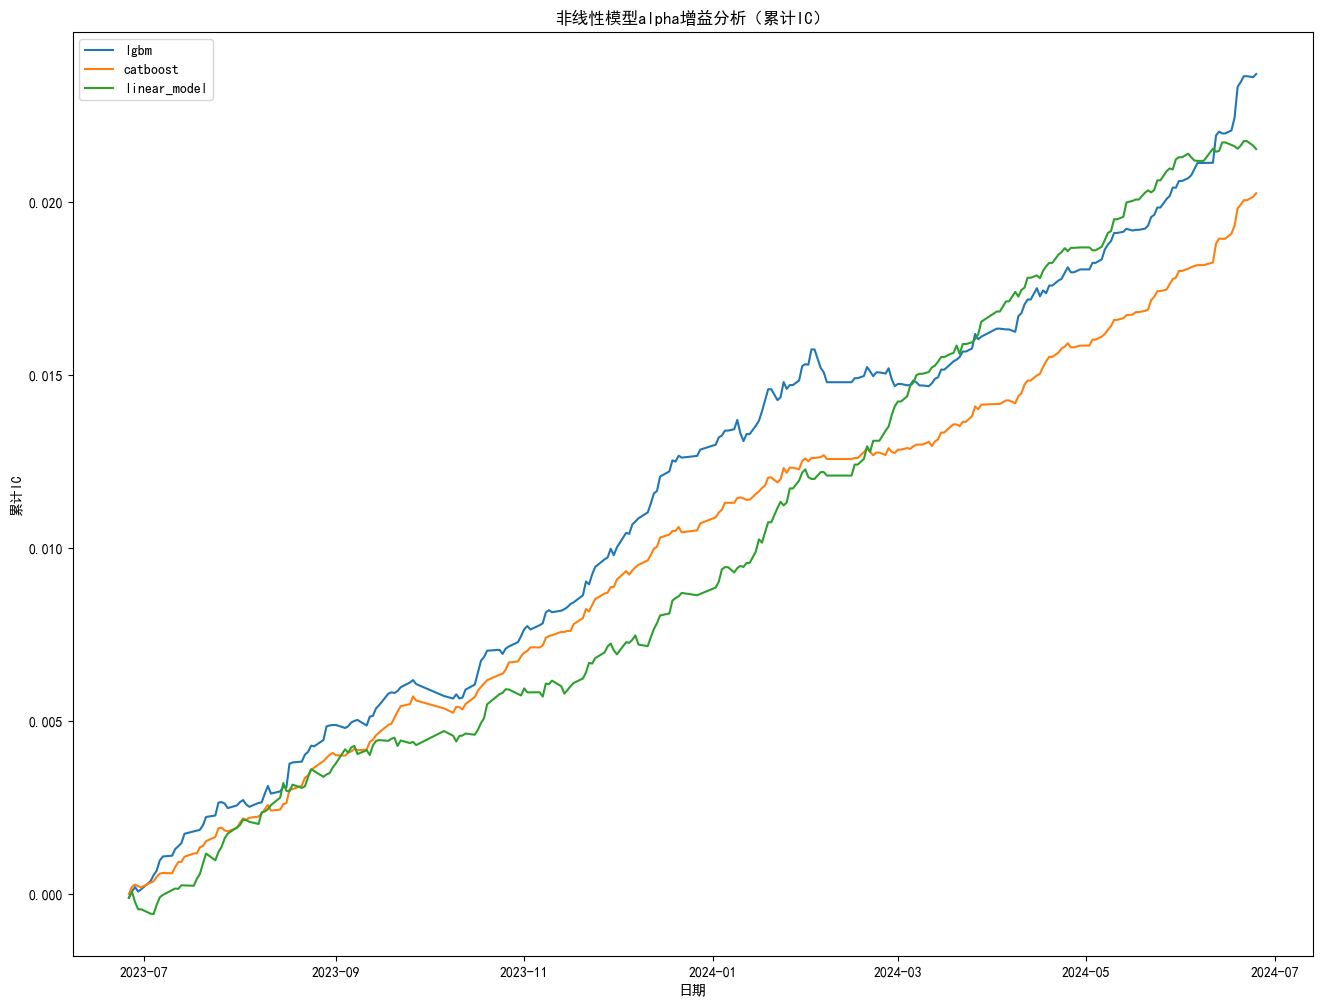
\includegraphics[width=0.88\linewidth,height=0.38\textheight,keepaspectratio]{../Figure/non-linear-outofsample.png}
    \vspace{-0.5em}
    {\tiny 样本外IC对比：非线性模型无显著增益}
\end{column}
\begin{column}{0.50\textwidth}
\textbf{七大核心发现}
\begin{enumerate}\setlength\itemsep{0pt}
    \item[\ding{172}] 北向资金具备\textbf{显著超额收益}（$\alpha$=0.0021, $t$=3.82）
    \item[\ding{173}] 收益以\textbf{择时为主}（58\%）而非选股
    \item[\ding{174}] 交易模式呈\textbf{"对冲基金式"高频}特征
    \item[\ding{175}] 预测力仅限\textbf{短期}，半年以上消失
    \item[\ding{176}] 引发约\textbf{一周的羊群效应}（$F$=15.44）
    \item[\ding{177}] DID证实标的股波动率\textbf{系统性上升}
    \item[\ding{178}] 策略alpha \textbf{SR$\approx$5.0}，与动量反转正交
\end{enumerate}

\vspace{0.1em}
\fcolorbox{red!70!black}{red!5}{%
\parbox{0.95\linewidth}{\centering\scriptsize
\textbf{"双刃剑"效应}：北向资金蕴含可挖掘的短期alpha，\\
但其高频交易\textbf{加剧}了A股短期波动，\\
对价格发现功能的促进作用\textbf{有限}。
}}
\end{column}
\end{columns}
\end{frame}

\end{document}
